%%% LaTeX Template: Two column assignment for BRSU
%%% Based on two column article from: http://www.howtotex.com/
%%% Preamble
\documentclass[	DIV=calc,%
				paper=a4,%
				fontsize=11pt,%
				twocolumn]{scrartcl}	 % KOMA-article class

\usepackage{lipsum}	% Package to create dummy text
\usepackage{blindtext}
\usepackage[english]{babel}	                          % English language/hyphenation
\usepackage[protrusion=true,expansion=true]{microtype} % Better typography
\usepackage{amsmath,amsfonts,amsthm}					 % Math packages
\usepackage[pdftex]{graphicx}	                          % Enable pdflatex
\usepackage[svgnames]{xcolor}	                          % Enabling colors by their 'svgnames'
\usepackage[hang, small,labelfont=bf,up,textfont=it,up]{caption} % Custom captions under/above floats
\usepackage{epstopdf}	 % Converts .eps to .pdf
\usepackage{subfig}	     % Subfigures
\usepackage{booktabs}	 % Nicer tables
\usepackage{fix-cm}       % Custom fontsizes
\usepackage{listings}
\usepackage{soul}
\usepackage{svg}
\usepackage{epstopdf}

%%% Custom sectioning (sectsty package)
\usepackage{sectsty}	 % Custom sectioning (see below)
\allsectionsfont{%% Change font of al section commands
	\usefont{OT1}{phv}{b}{n}%% bch-b-n: CharterBT-Bold font
	}

\sectionfont{%% Change font of \section command
	\usefont{OT1}{phv}{b}{n}%% bch-b-n: CharterBT-Bold font
	}


\definecolor{brsugrey}{rgb}{0.9, 0.9, 0.9}
\definecolor{brsublue}{rgb}{0, 0.594, 0.949}


\newcommand{\upperRomannumeral}[1]{\uppercase\expandafter{\romannumeral#1}}

%%% Headers and footers
\usepackage{fancyhdr} % Needed to define custom headers/footers
	\pagestyle{fancy} % Enabling the custom headers/footers
\usepackage{lastpage}	

% Header (empty)
\lhead{}
\chead{}
\rhead{}
% Footer (you may change this to your own needs)
\lfoot{\footnotesize 
\texttt{LAA} % Set to the course abbreviation 
\textbullet ~ Hagg % Set to your name
\textbullet ~ Assignment \upperRomannumeral{2}} % Set the assignment number
\cfoot{}
\rfoot{\footnotesize page \thepage\ of \pageref{LastPage}}	% "Page 1 of 2"
\renewcommand{\headrulewidth}{0.0pt}
\renewcommand{\footrulewidth}{0.4pt}



%%% Creating an initial of the very first character of the content
\usepackage{lettrine}
\newcommand{\initial}[1]{%
     \lettrine[lines=3,lhang=0.3,nindent=0em]{
     				\color{brsublue}
     				{\textsf{#1}}}{}}

%%% Title, author and date metadata
\usepackage{titling}	% For custom titles

\newcommand{\HorRule}{\color{brsublue}% Creating a horizontal rule
					 \rule{\linewidth}{1pt}%
					 \color{black}
					 }

\pretitle{\vspace{-30pt} \begin{flushleft} \HorRule 
				\fontsize{25}{25} \usefont{OT1}{phv}{b}{n} \color{gray} \selectfont 
				}
\title{Learning and Adaptivity
\\ Assignment ~\upperRomannumeral{2}}% Title of your article goes here
\posttitle{\par\end{flushleft}\vskip 0.5em}

\preauthor{\begin{flushleft}
\large \lineskip 0.25em \usefont{OT1}{phv}{b}{sl} \color{brsublue}}
\author{Alexander Hagg, Adam Gaier }	% Author name goes here
\postauthor{\footnotesize \usefont{OT1}{phv}{m}{sl} \color{Black} 
BRS University of Applied Sciences % Institution of author
\\email: alexander.hagg@smail.inf.h-brs.de ~github: @alexander-hagg
\par\end{flushleft}\HorRule}

\date{\today} 

%%% Begin document
\begin{document}
\maketitle
\thispagestyle{fancy} % Enabling the custom headers/footers for the first page 
% The first character should be within \initial{}
\initial{D}\textbf{ } ecision tree learning is used to learn concepts or other discrete-valued functions. It allows building a short tree where nodes represent a decision, based on the value of a certain parameter, which has to be defined for all data tuples. 

\setcounter{section}{5}
\section{Decision Tree Learning}
\subsection{Simple Prediction}

\begin{enumerate}
	\item Predicting animal type from all other attributes (except for the species' name). Two decision trees were built using all data from the zoo database. The next best attribute was chosen using two available methods: gini index and entropy. The gini index on a data set T is defined as $\mathrm{gini(T)} := 1 - \sum_i p_i^2$\footnote{Taken from lecture notes from the "Knowledge Extraction and Machine Learning" course at the University of Porto, http://paginas.fe.up.pt/\textasciitilde ec/}, where $p_i$ is the relative frequency of class $i$. The entropy measure measures the impurity of sample S of training examples. 
	As can be taken from the results in \ref{7-1-gini} and \ref{7-1-entropy}, they differ in the sense that using the entropy split criterion tends to be a bit more conservative and gini tends to pick and split larger classes faster.
	
	\item Predicting animal type from all other attributes (including the species' name). As can be taken from the results in \ref{7-2-gini} and \ref{7-2-entropy}, including the name of the animal, which is unique for every animal, obviously does not help in classification.
	
	\item Predicting, whether an animal is airborne, from all other attributes (including type, excluding name). Results can be taken from figure \ref{7-3-gini}. The attributes "feathers", "domestic" and "fins" are the first three best splitters, according to the gini criterion, which leads to large categories being split earlier on in the process.
	
	\item Predicting species' name from all other attributes. Figure \ref{7-4-gini} shows that some groups of animals cannot be distinguished, because they have the same attributes. This is shown by the leaves' gini value being greater than zero (the relative frequency of the members of the "class" is not 1).
\end{enumerate}

\subsection{Scalability}

\begin{enumerate}
	\item As we do not use the applet, we did not run into any problems performance wise, as we can choose not to visualize.
	\item We were not able to visualize the decision trees for training sets large than 200 samples. This issue is known by the TA. Instead, we decided to display the number of nodes in the tree to get a grasp on the size of it. As can be taken from figure \ref{8-2-performance}, the number of nodes is near linear to the percentage of total data used for training. The time taken is linear as well. The top figure in figure \ref{8-2-performance} shows the mean error rate on the test set, with the blue region representing the standard deviation of the error. We can see that the error mean goes down until approximately 70\% of the data is used for training. After that, a plateau occurs and eventually the error rate (and especially its standard deviation) goes up again, which is probably caused by overfitting.
	 Figure \ref{8-1-error} shows the error rate mean and standard deviation for the individual letters. 
\end{enumerate}

\subsection{Noise}

Data preprocessing algorithm:
\begin{enumerate}
	\item Sort and split data in 'letter' groups
		\begin{enumerate}
		\item For all groups: get the 'mean' letter (using k-means, or by just taking the median)	
		\end{enumerate}
		\begin{enumerate}
		\item For all letters (and their supposed category label):
			\begin{enumerate}
			\item The noise is defined as the euclidean distance to the mean of its category
			\item If the distance is smaller than than a certain innerclass noise threshold, e.g. twice the standard deviation of the group, we call this innerclass noise. We assume the label is correct and the distance to the mean is caused by the variance within the group.
			\item If the distance is greater than a certain outerclass noise threshold, e.g. twice the standard deviation, we call this intraclass noise.
			\end{enumerate}
		\end{enumerate}
\end{enumerate}

\begin{itemize}
	\item Noise(group i) = The number of noisy instances / number of nonnoisy instances * 100\% 
	\item Noise is now controlled by picking a certain number of noisy instances and a number of nonnoisy instances. The intraclass noise can be separately controlled by instead of taking "the number of noisy instances", taking "number of noisy inner class instances + number of noisy intraclass instances"
	\item A refined noise quantization could weight the noisy instances by their actual distance to the mean.
\end{itemize}
	 
\vfill

\section*{Conclusion}

The assignment definitely got improved by giving us the opportunity to use Python instead of a preprogrammed Java applet. But instead of taking two different databases, the assignment could be reduced to just the letter database, and instead increase the "in-depth" on e.g. overfitting and when this happens. Writing an algorithm to determine the noise was done by us, but there was absolutely no time left to actually implement and analyze its results. 

\section*{Sources}

Theory: http://paginas.fe.up.pt/\textasciitilde ec/

Code snippets: from our TA. 

\newpage

\onecolumn
\section*{Appendix A: Code}

\HorRule

\lstinputlisting[language=Python, numbers=left, firstline=51, 
				lastline=61, frame=L, title=\lstname]{code/zoo_ml.py}

\HorRule

\lstinputlisting[language=Python, numbers=left, firstline=59, 
				lastline=106, frame=L, title=\lstname]{code/letters_ml.py}
				
\HorRule

Visualization and data analysis in MATLAB:

\lstinputlisting[language=Matlab, numbers=left, firstline=2, 
				lastline=65, frame=L, title=\lstname]{code/letter_data.m}

\newpage


\section*{Appendix B: Results}

\HorRule

\begin{figure}[h]
  \centering
  \caption{Decision tree predicting animal type}
  \label{7-1-gini}
  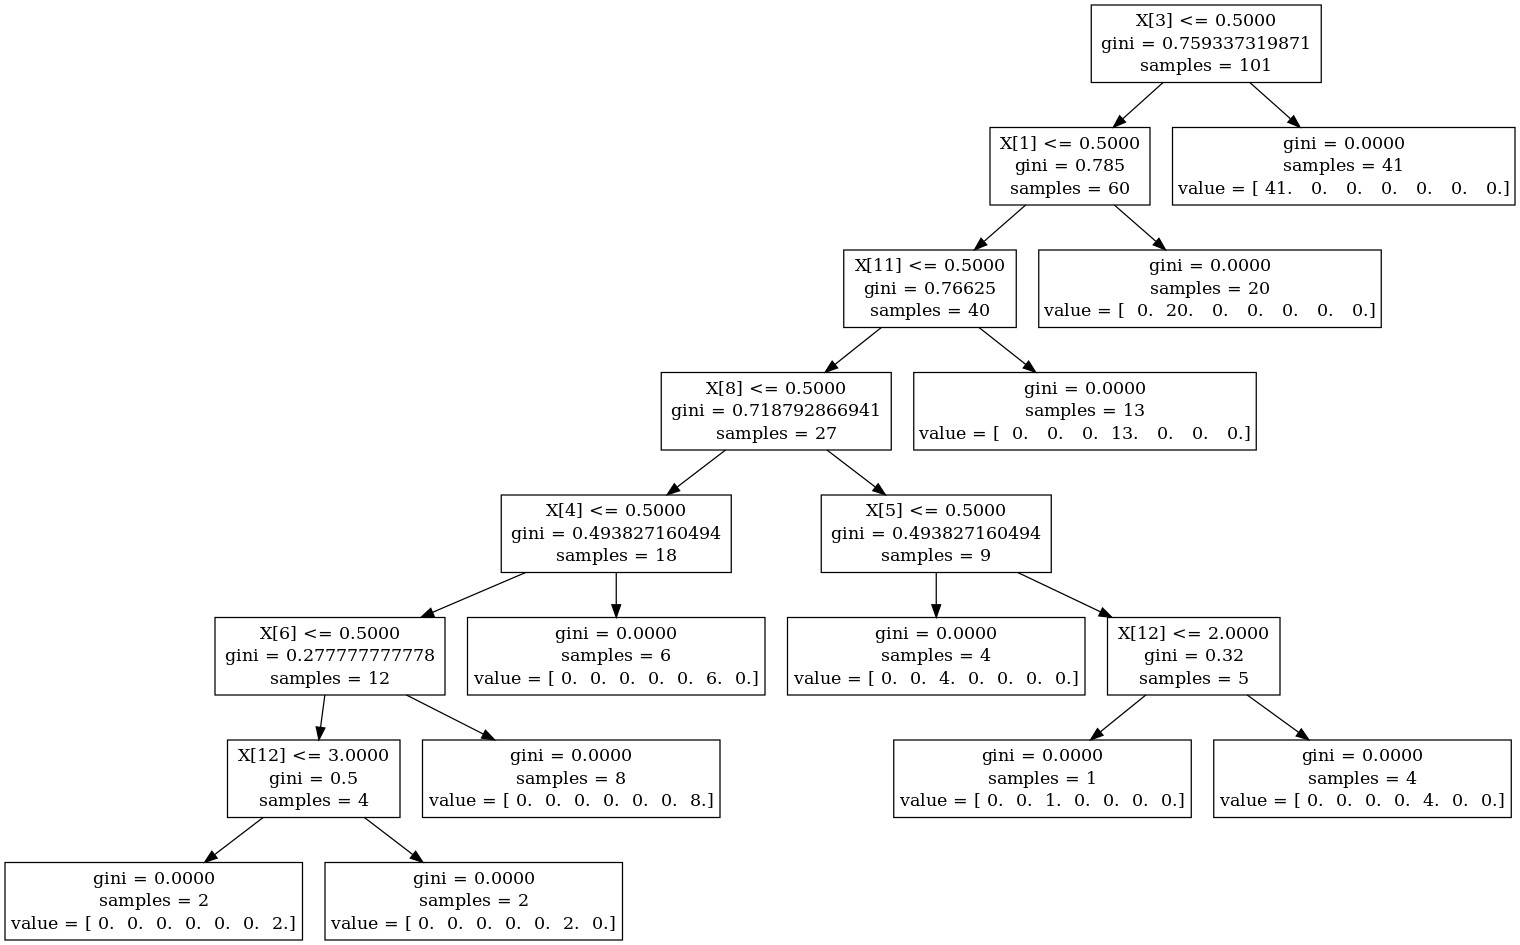
\includegraphics[width=1\textwidth]{./img/7-1-gini.jpg}
\end{figure}

\begin{figure}[h]
  \centering
  \caption{Decision tree predicting animal type}
  \label{7-1-entropy}
  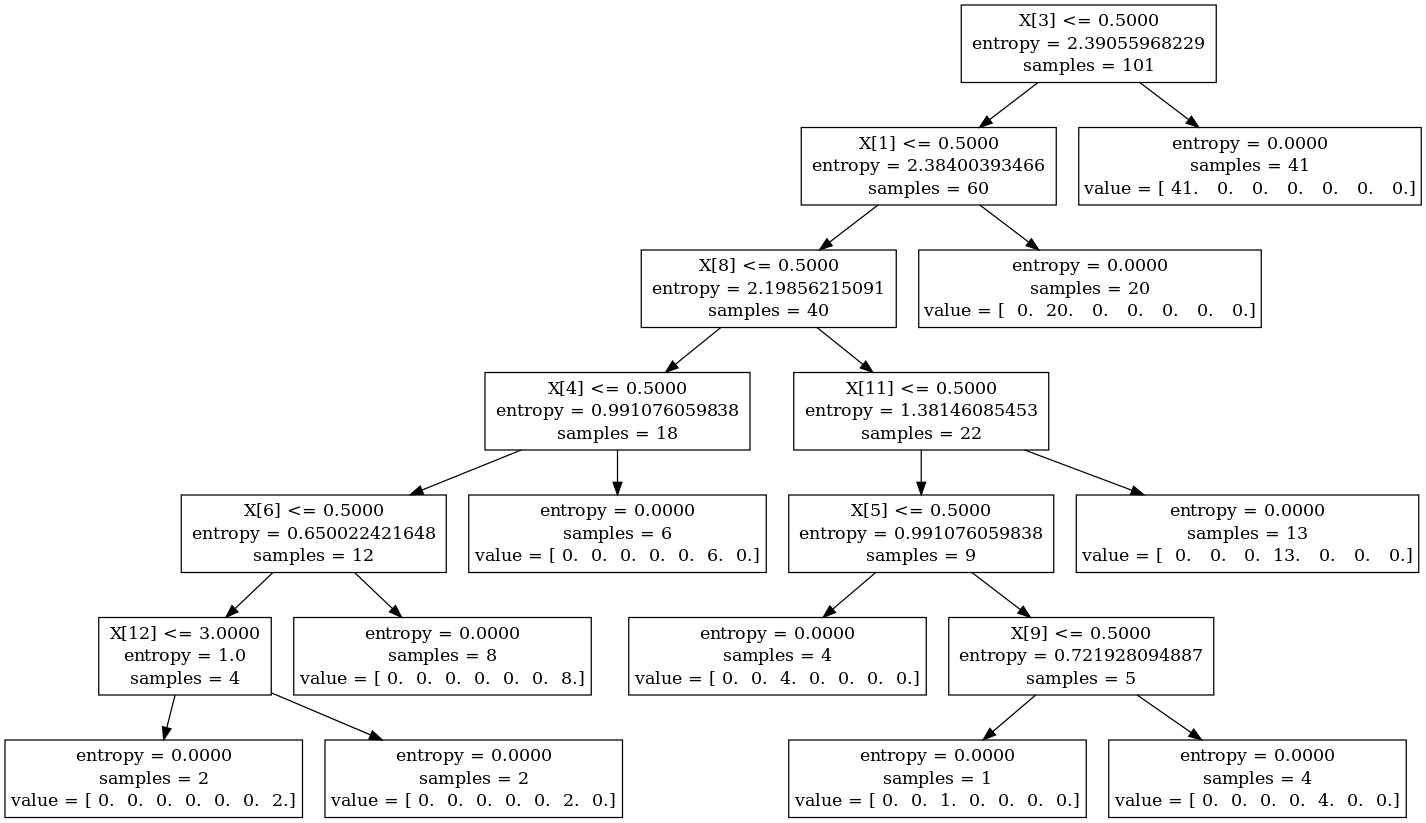
\includegraphics[width=1\textwidth]{./img/7-1-entropy.jpg}
\end{figure}

\begin{figure}[h]
  \centering
  \caption{Decision tree predicting animal type incl. name}
  \label{7-2-gini}
  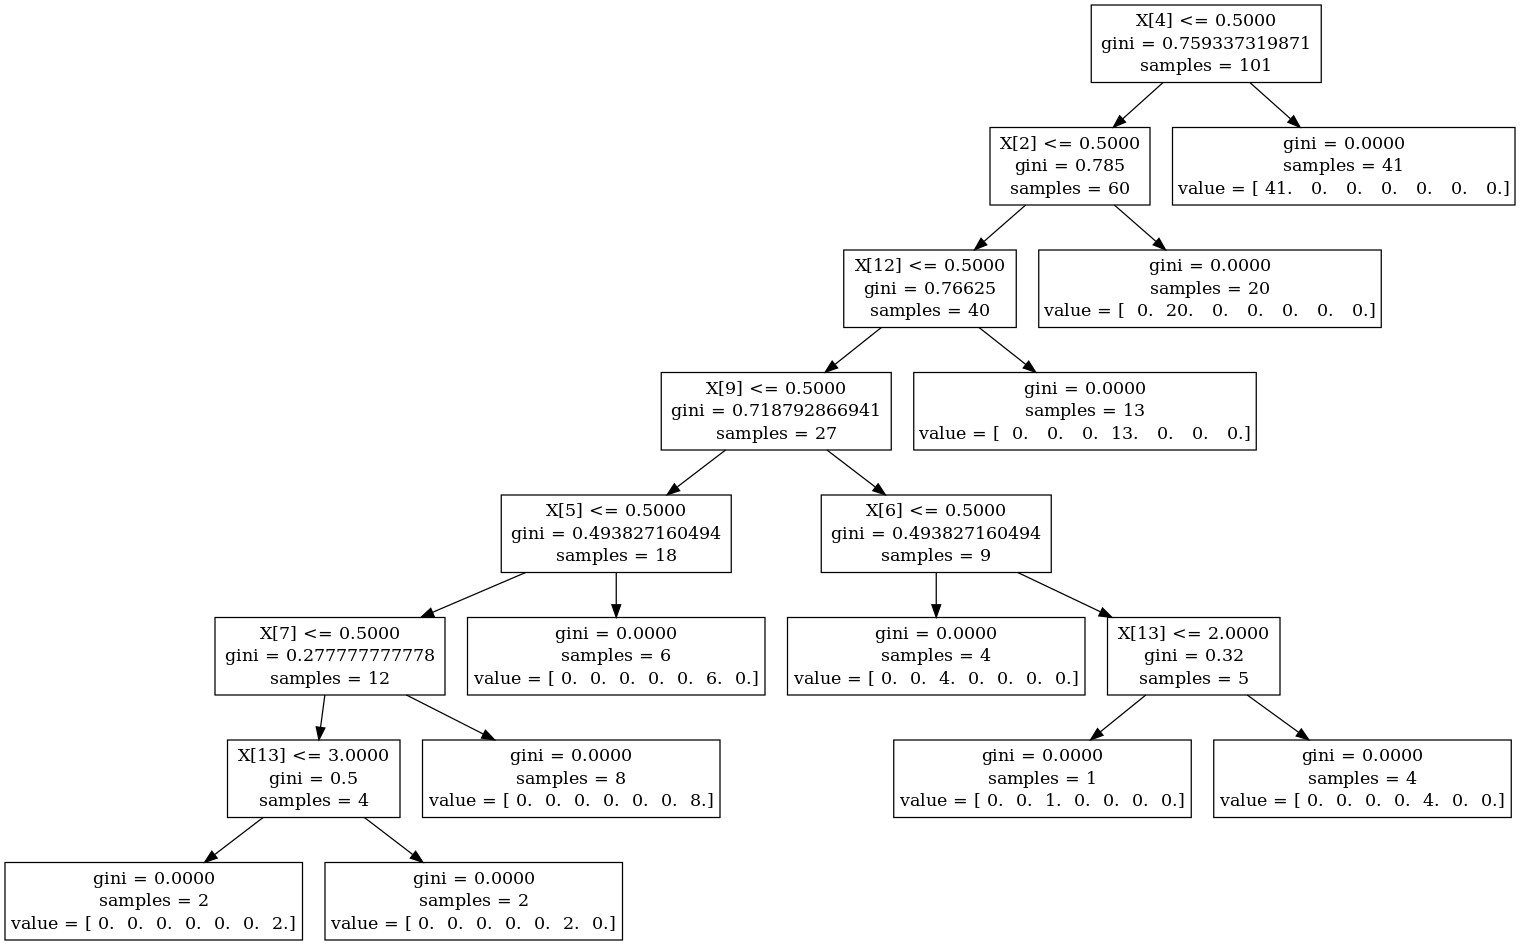
\includegraphics[width=1\textwidth]{./img/7-2-gini.jpg}
\end{figure}

\begin{figure}[h]
  \centering
  \caption{Decision tree predicting animal type incl. name}
  \label{7-2-entropy}
  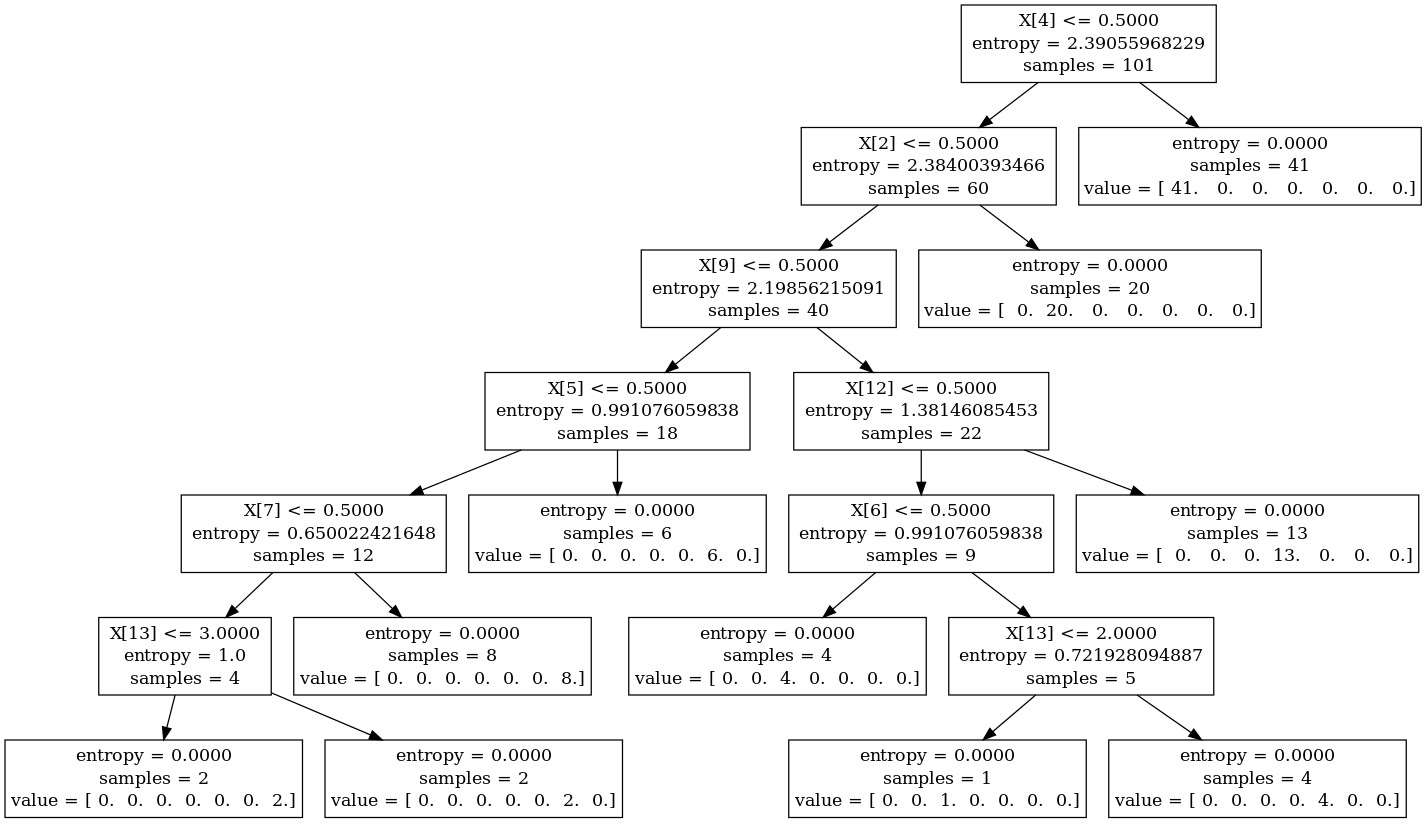
\includegraphics[width=1\textwidth]{./img/7-2-entropy.jpg}
\end{figure}

\begin{figure}[h]
  \centering
  \caption{Decision tree predicting whether animal is airborne}
  \label{7-3-gini}
  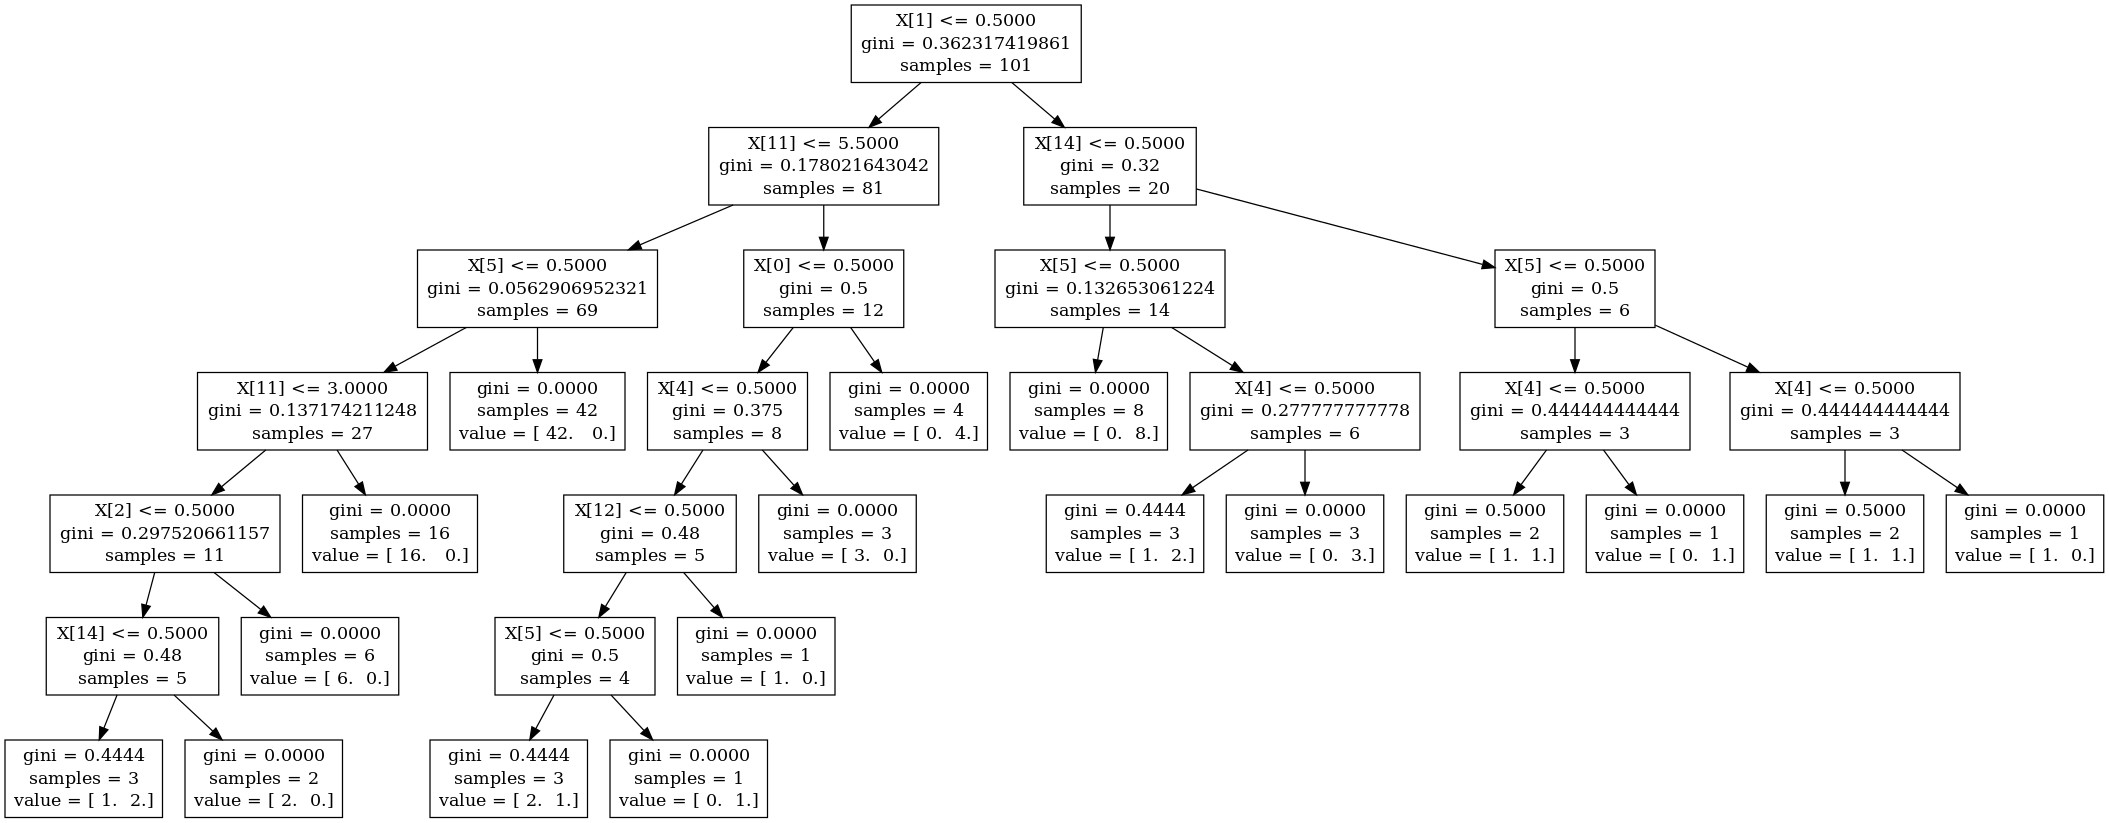
\includegraphics[width=1\textwidth]{./img/7-3-gini.jpg}
\end{figure}

\begin{figure}[h]
  \centering
  \caption{Decision tree predicting animal name}
  \label{7-4-gini}
  
\includegraphics[width=1\textwidth]{./img/7-4-gini.jpg}
\end{figure}

\begin{figure}[h]
  \centering
  \caption{Decision tree predicting letters: mean letter error rates}
  \label{8-1-error}
  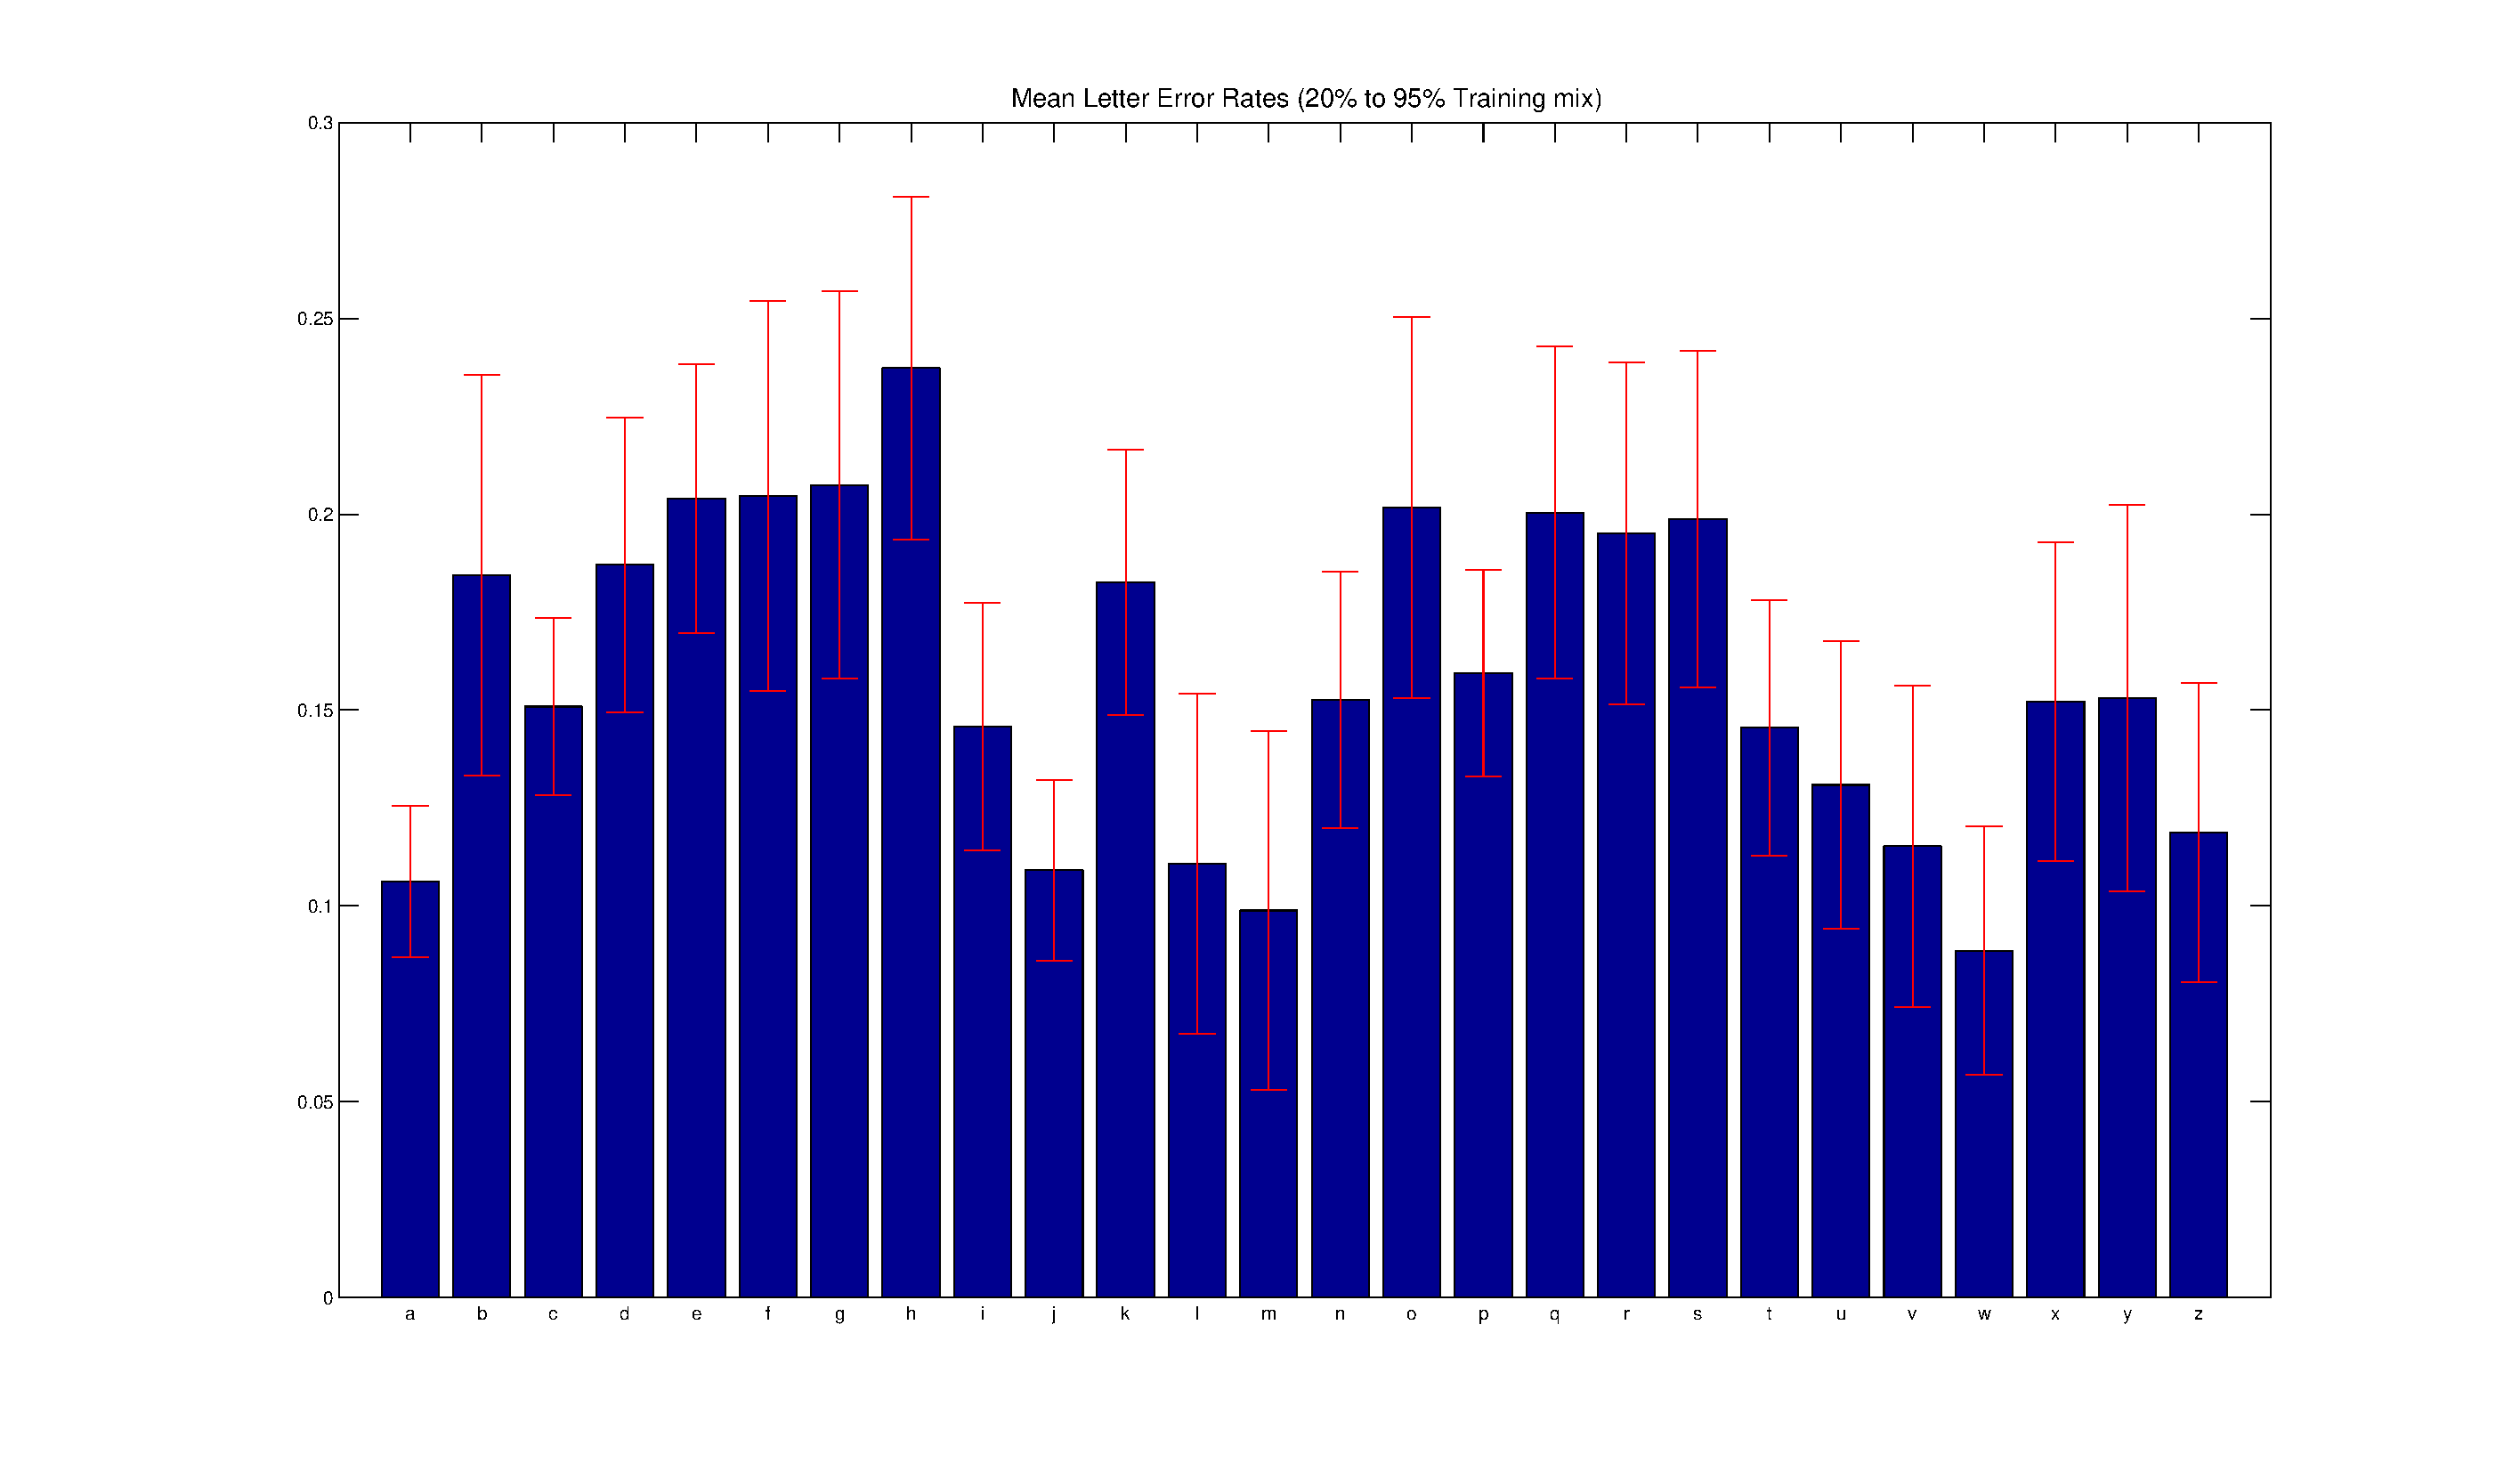
\includegraphics[width=1\textwidth]{./img/letter_error.eps}
\end{figure}

\begin{figure}[h]
  \centering
  \caption{Performance on letters}
  \label{8-2-performance}
  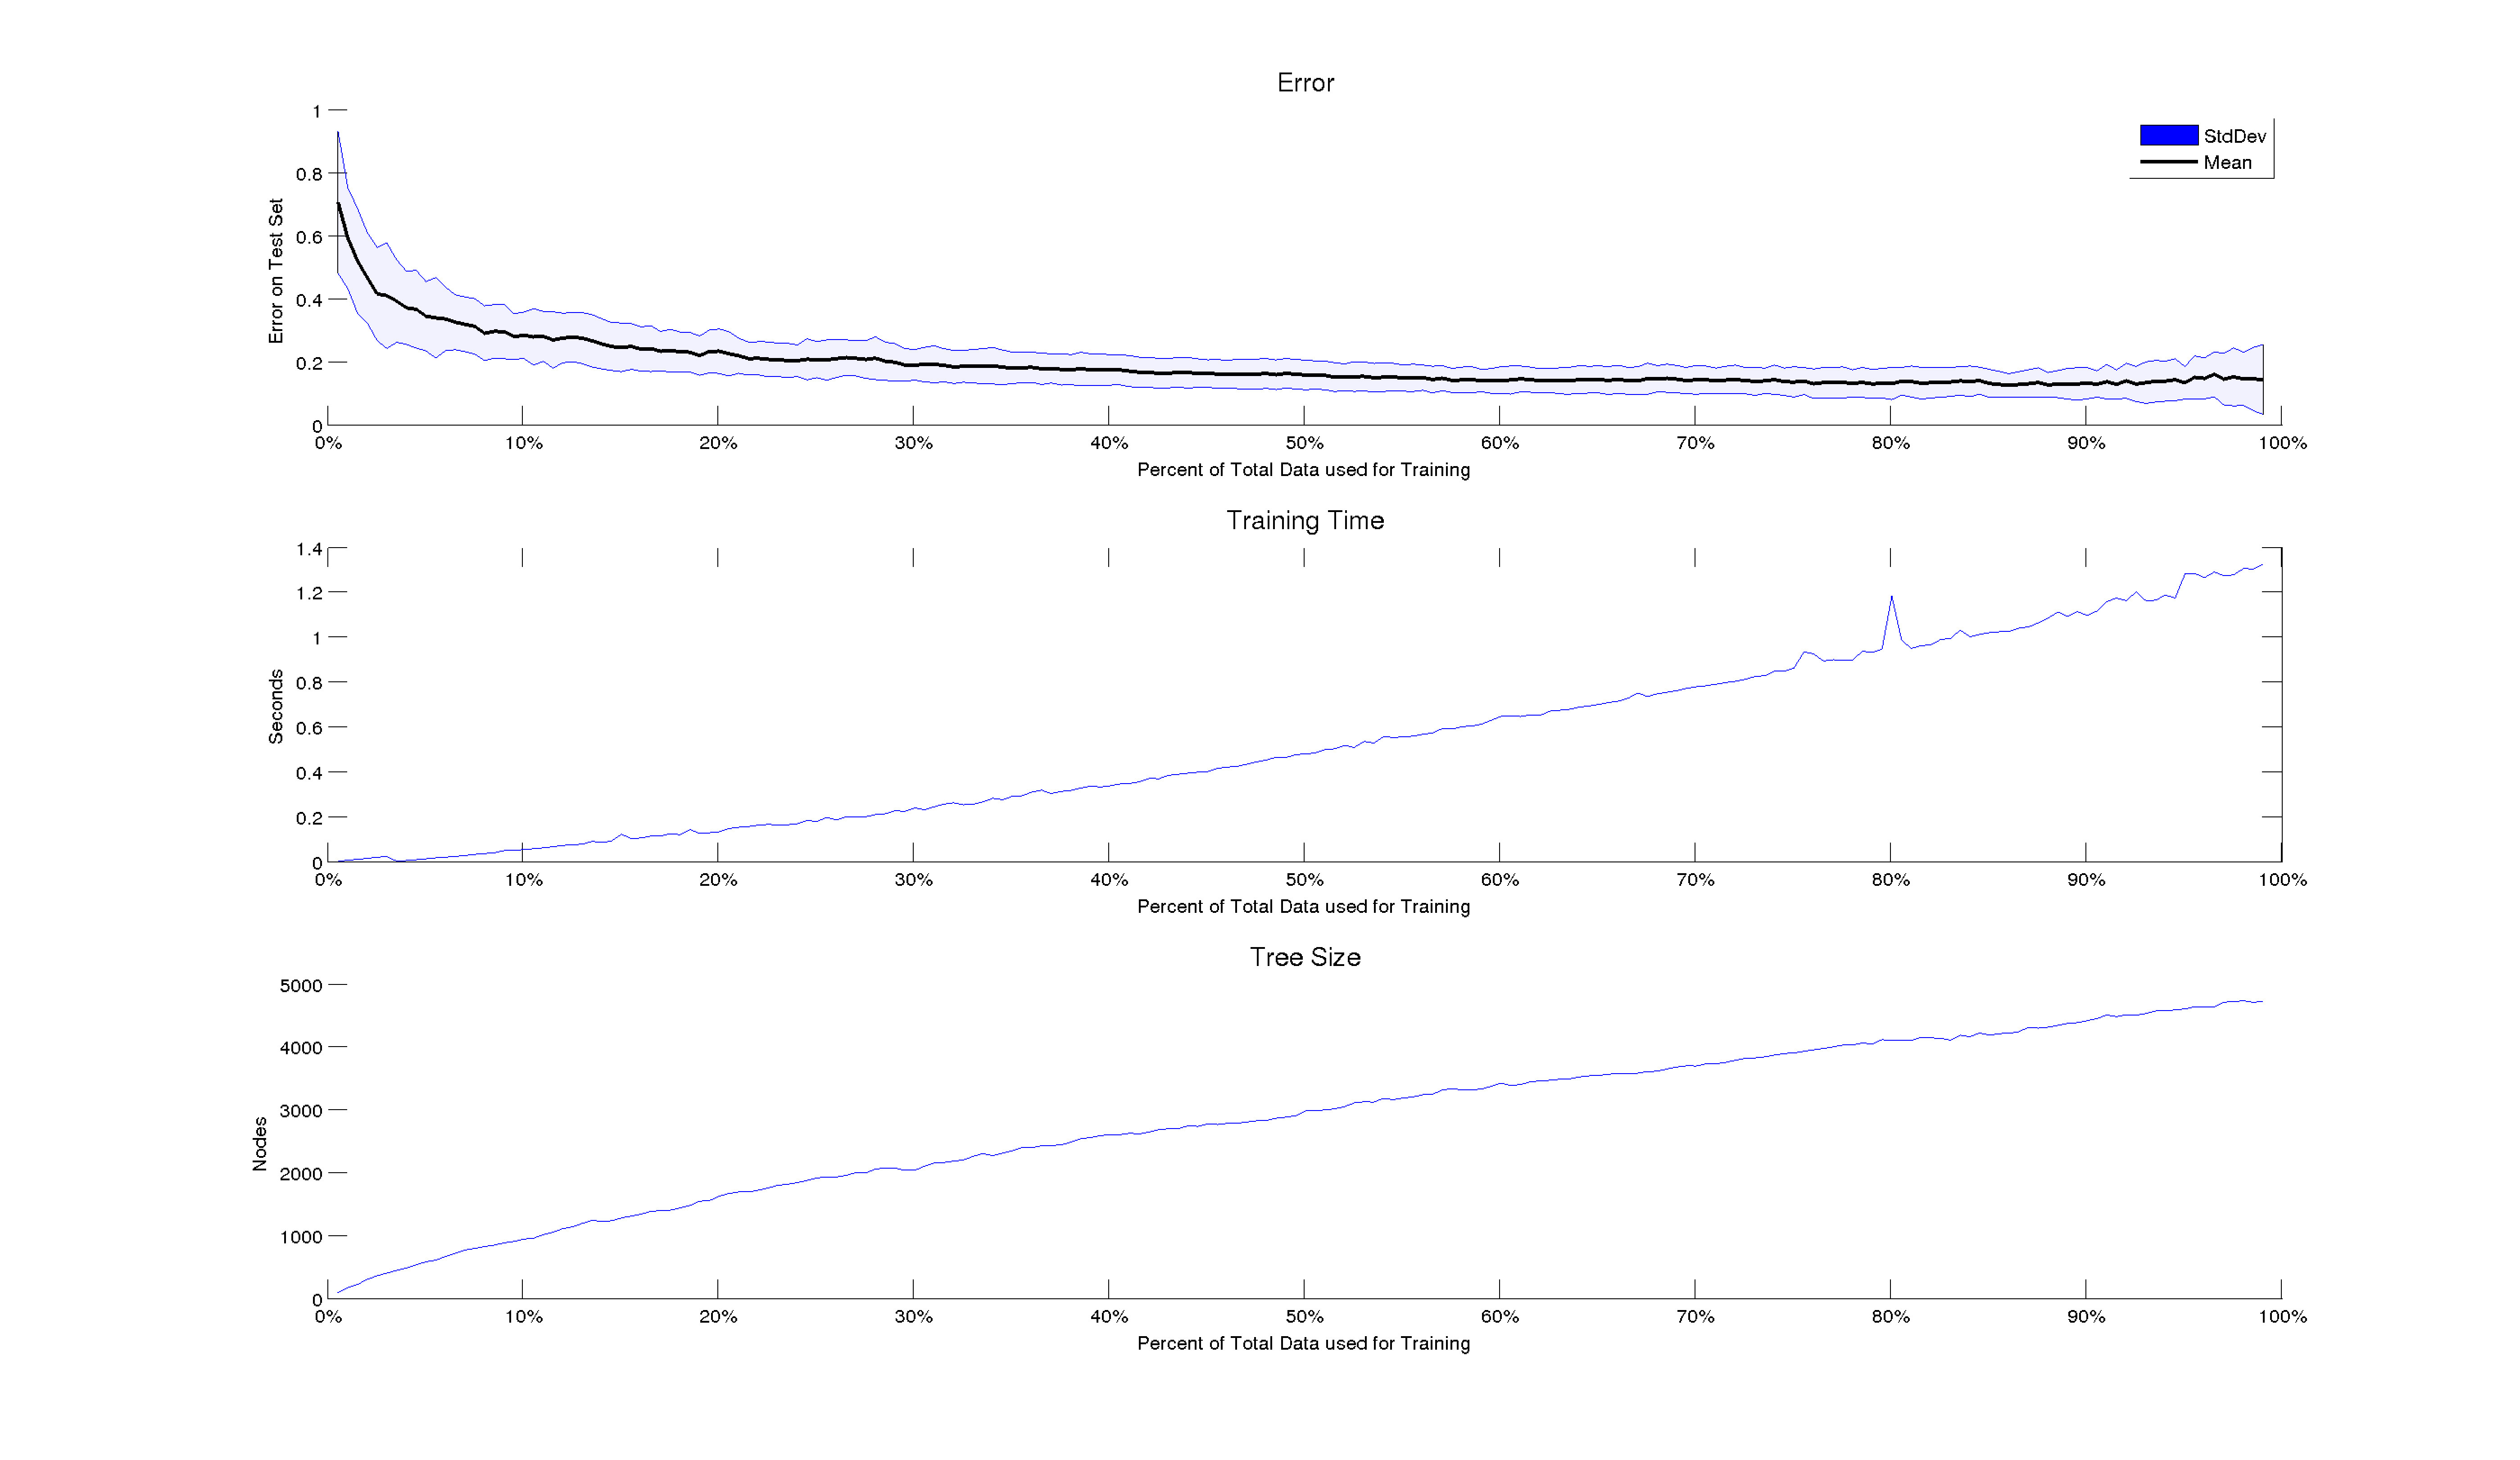
\includegraphics[width=1\textwidth]{./img/performance.eps}
\end{figure}
\end{document}